\section{Strava API}

\begin{frame}{API v.s. UI}
\begin{center}
\begin{tabular}{c|c}
API (Application Program Interface) & UI (User Interface)\\
應用程式介面 & 使用者介面\\\hline\pause
無須了解伺服器內部的程式如何運作 & 無須了解伺服器內部的程式如何運作\\\pause
讓開發者可以更輕易的跟伺服器互動 & 讓使用者可以更輕易的跟伺服器互動\\\pause
GET, POST requests, formatted response & 網頁、地圖、圖表、按鈕\\\pause
Access token & Cookie
\end{tabular}
\end{center}
\end{frame}

\begin{frame}{API v.s. UI}
\begin{itemize}
\item 我要 TBA 四極點活動的資料:\pause
\begin{multicols}{2}
\item API:\\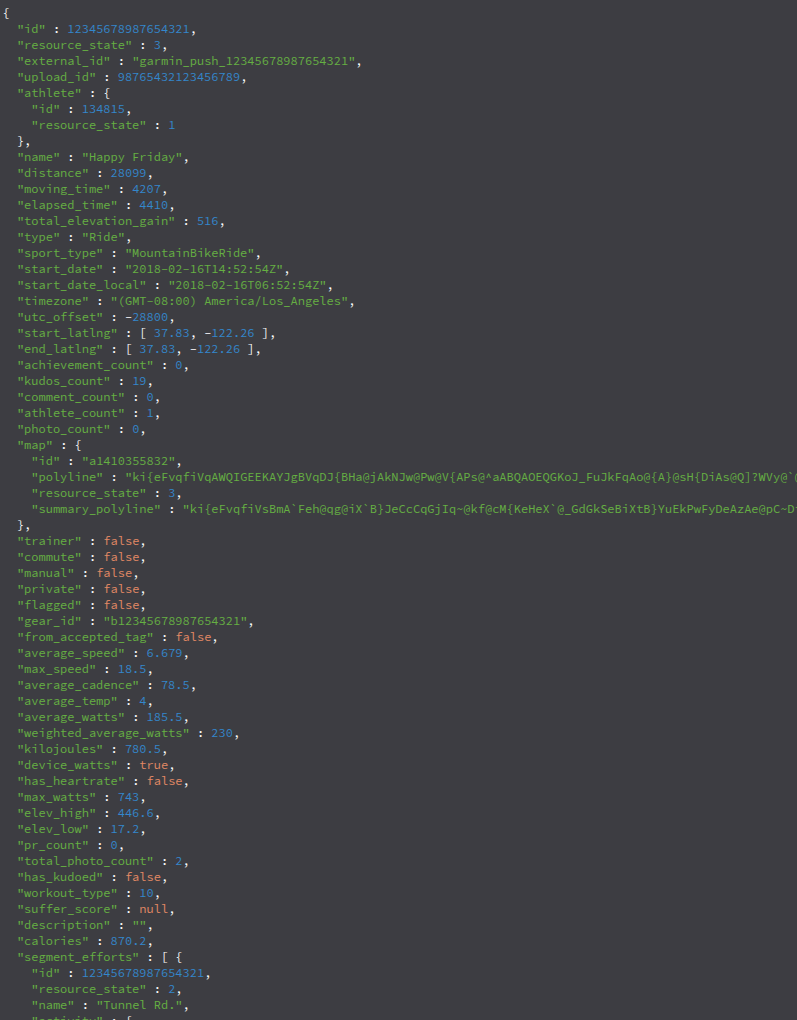
\includegraphics[height=6cm]{API.png}
\newpage
\item UI:\\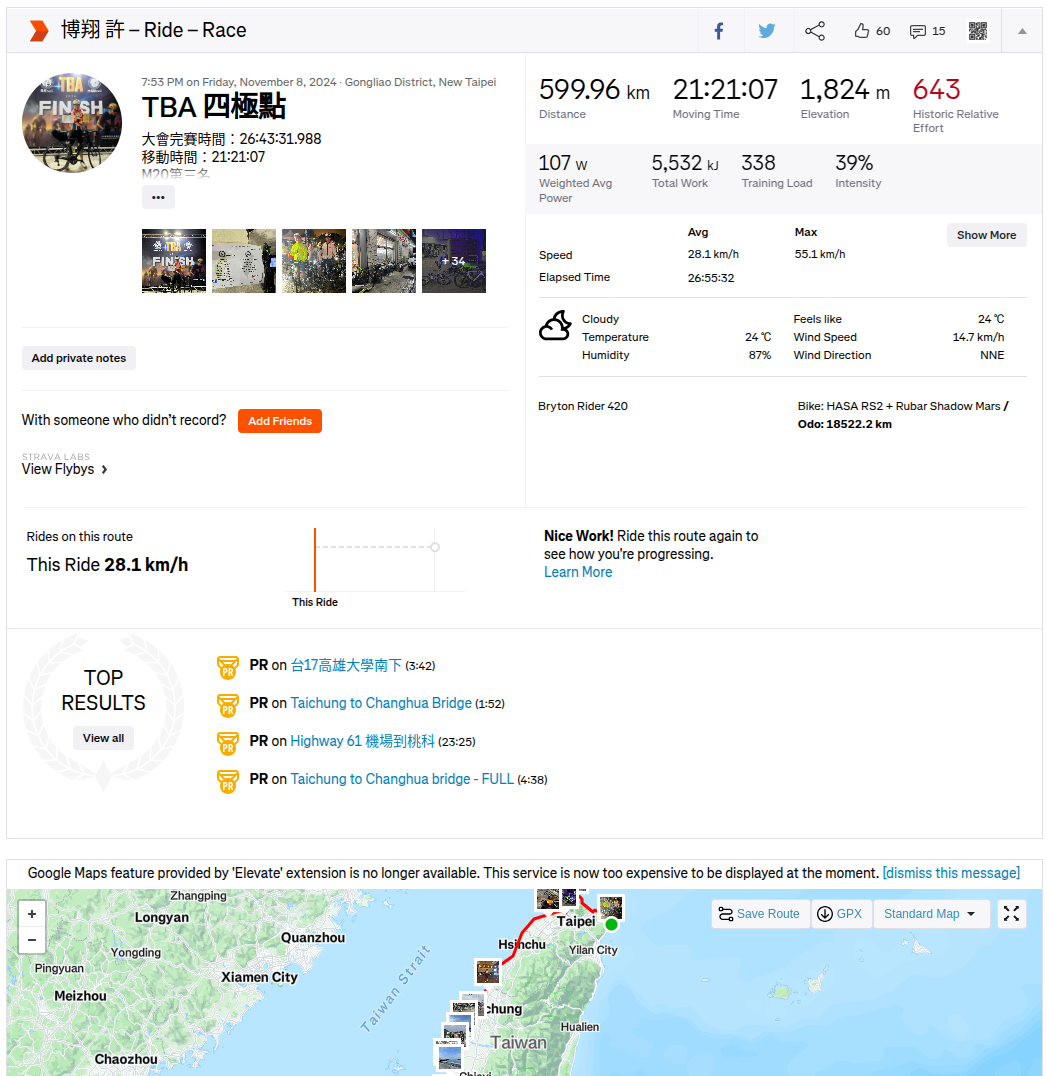
\includegraphics[height=6cm]{UI.png}
\end{multicols}
\end{itemize}
\end{frame}

\begin{frame}{Create An Application}
\begin{itemize}
\item \href{https://www.strava.com/settings/api}{My API Application}\\
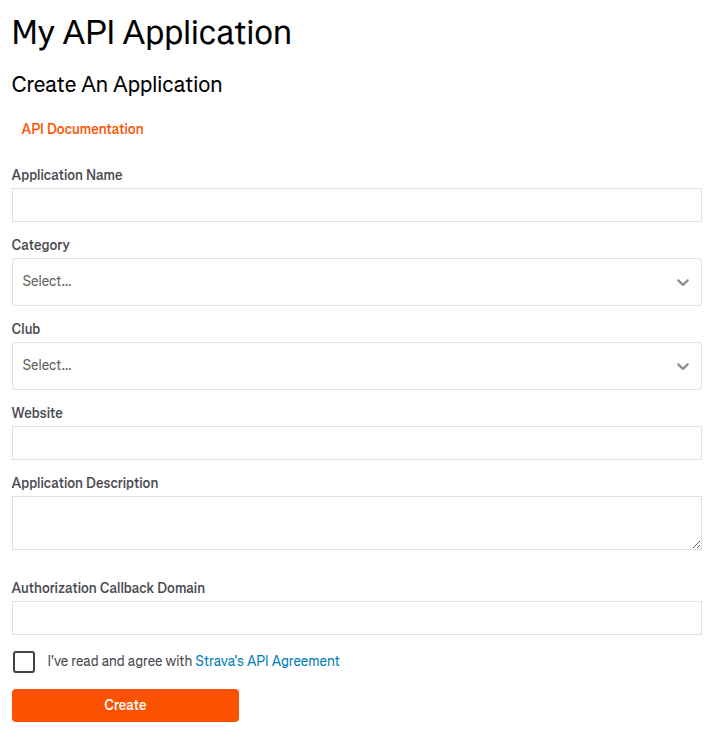
\includegraphics[height=7cm]{createAPI.png}
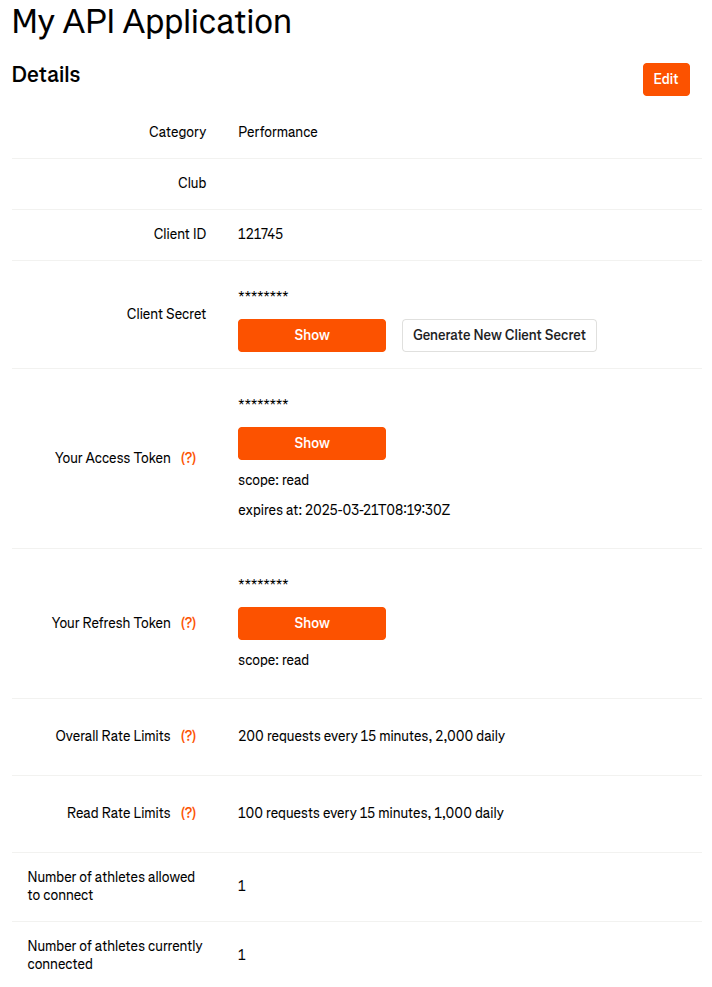
\includegraphics[height=7cm]{createAPI2.png}
\end{itemize}
\end{frame}

\begin{frame}{Get Access Permission}
\begin{itemize}
\item 你(A)想取用某個人(B)的資料
\item Strava 要判斷:
\begin{itemize}
\item 你真的是A: Strava 要看你的\texttt{client\_id}與\texttt{client\_secret}是否吻合
\item 而且B同意:讓使用者進入同意你的取用的頁面,按下同意後產生的\texttt{code}就是使用者同意的證明
\end{itemize}
\item 拿著\texttt{client\_id}、\texttt{client\_secret}、\texttt{code}一起跟 Strava 要權限, Strava 會給你一個暫時證明你有權限的 token\\
\only<1>{
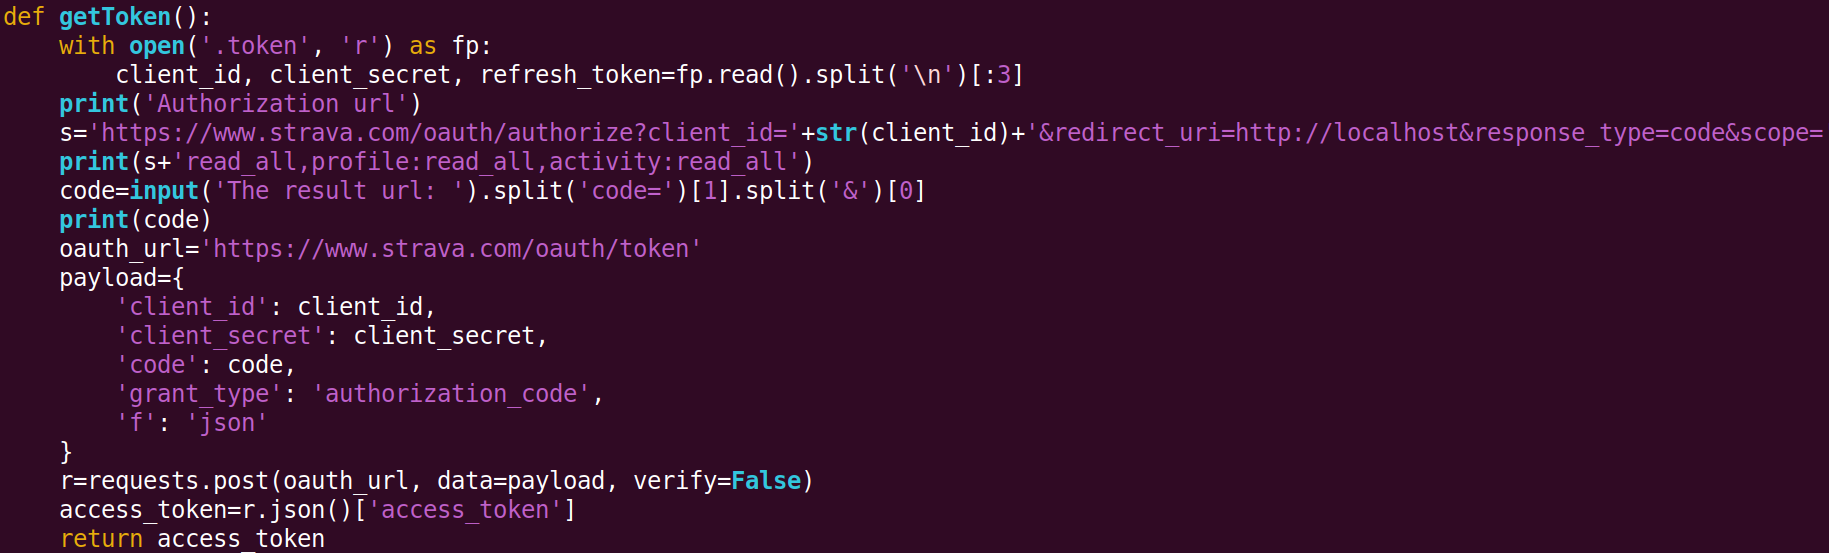
\includegraphics[height=4cm]{authorize0.png}
}\only<2>{
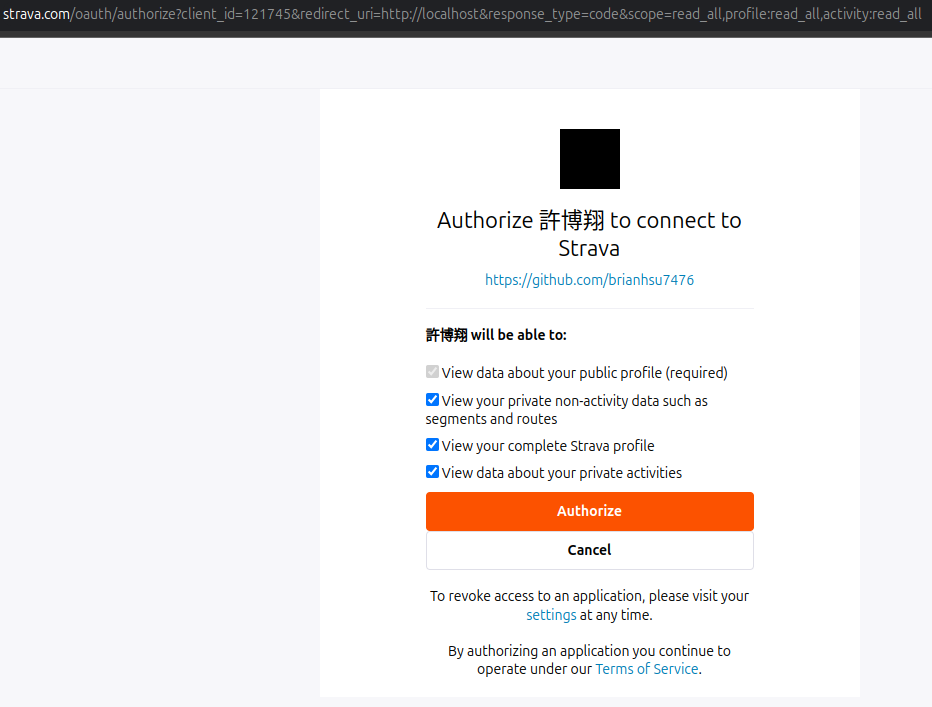
\includegraphics[height=3cm]{authorize1.png}
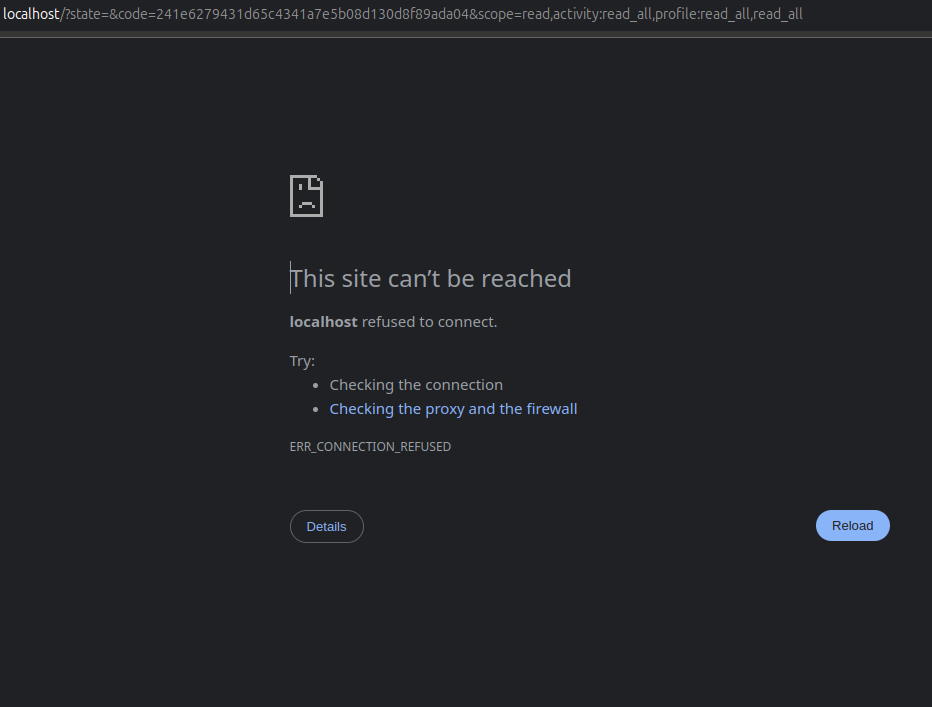
\includegraphics[height=3cm]{authorize2.png}
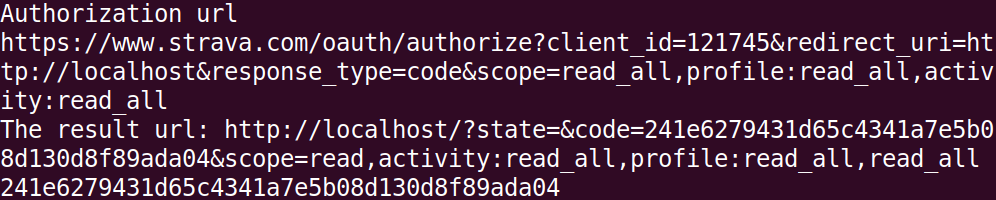
\includegraphics[width=7cm]{authorize3.png}
}
\end{itemize}
\end{frame}

\begin{frame}{Get Data}
\begin{itemize}
\item \href{https://developers.strava.com/docs/reference/}{Documentation}
\item 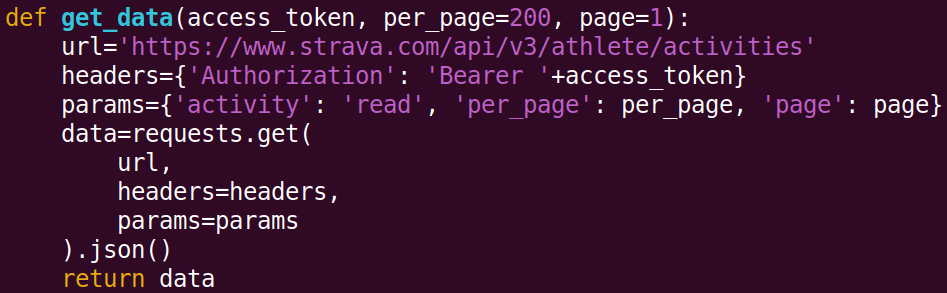
\includegraphics[width=14cm]{getActivity.png}
\end{itemize}
\end{frame}

\begin{frame}{Some Projects}
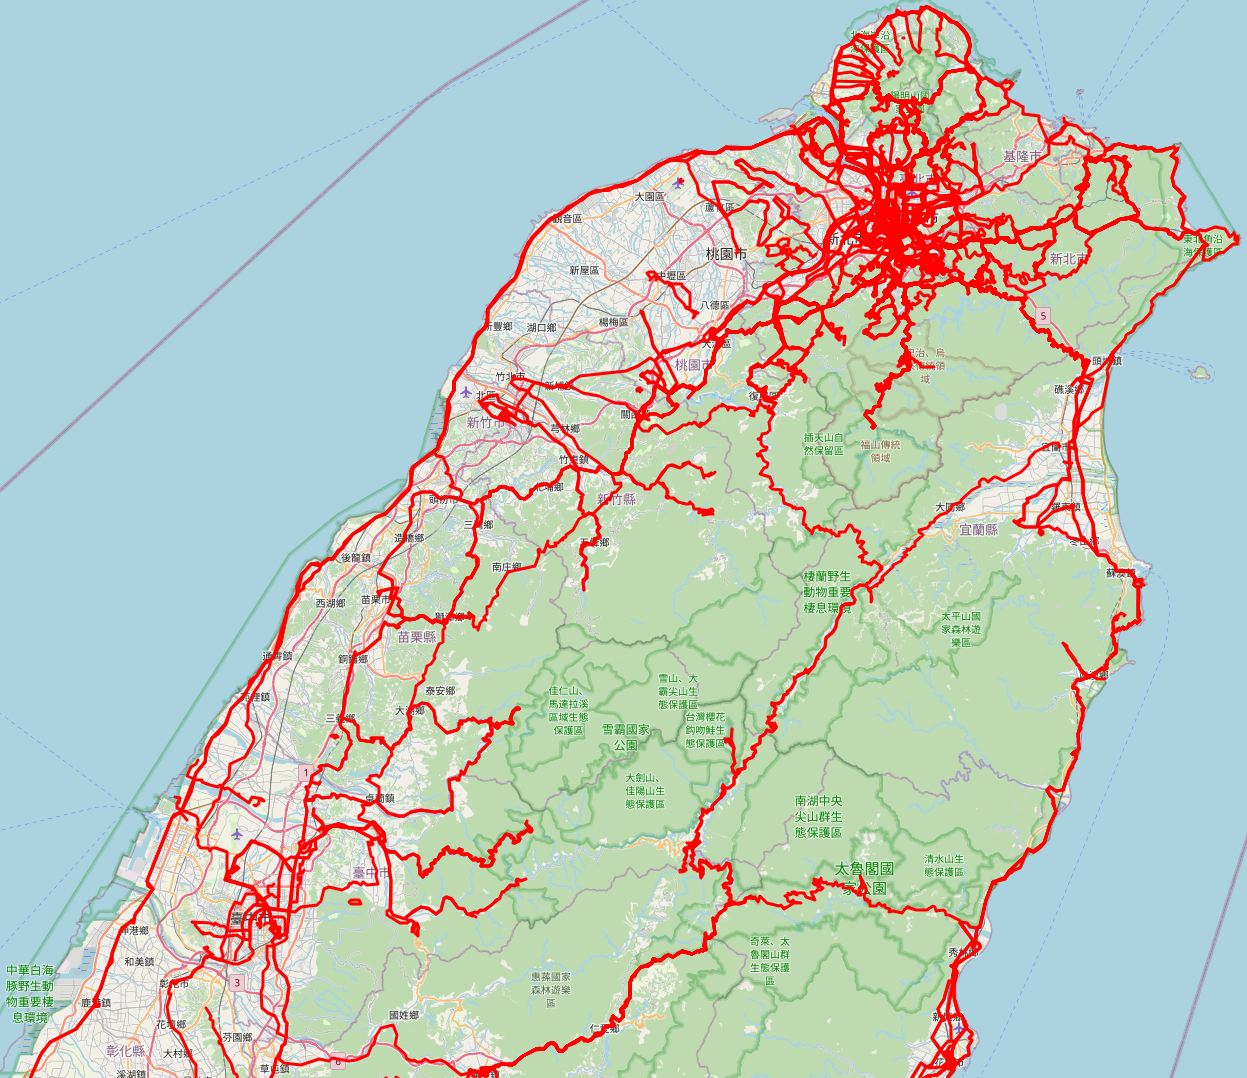
\includegraphics[height=4cm]{apiHeatMap.png}\pause
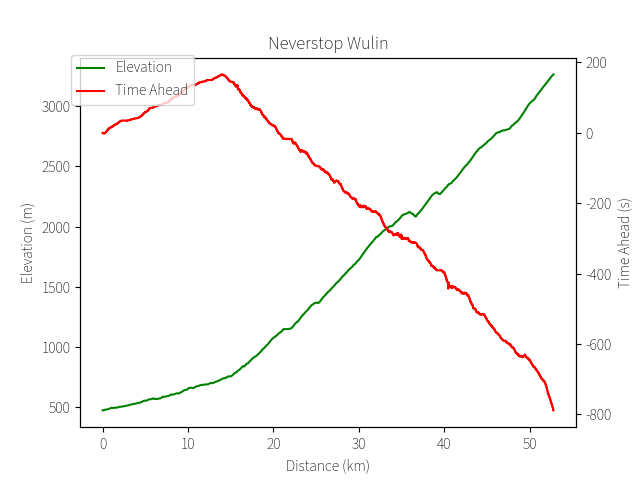
\includegraphics[height=4cm]{NeverstopWuling.png}\pause
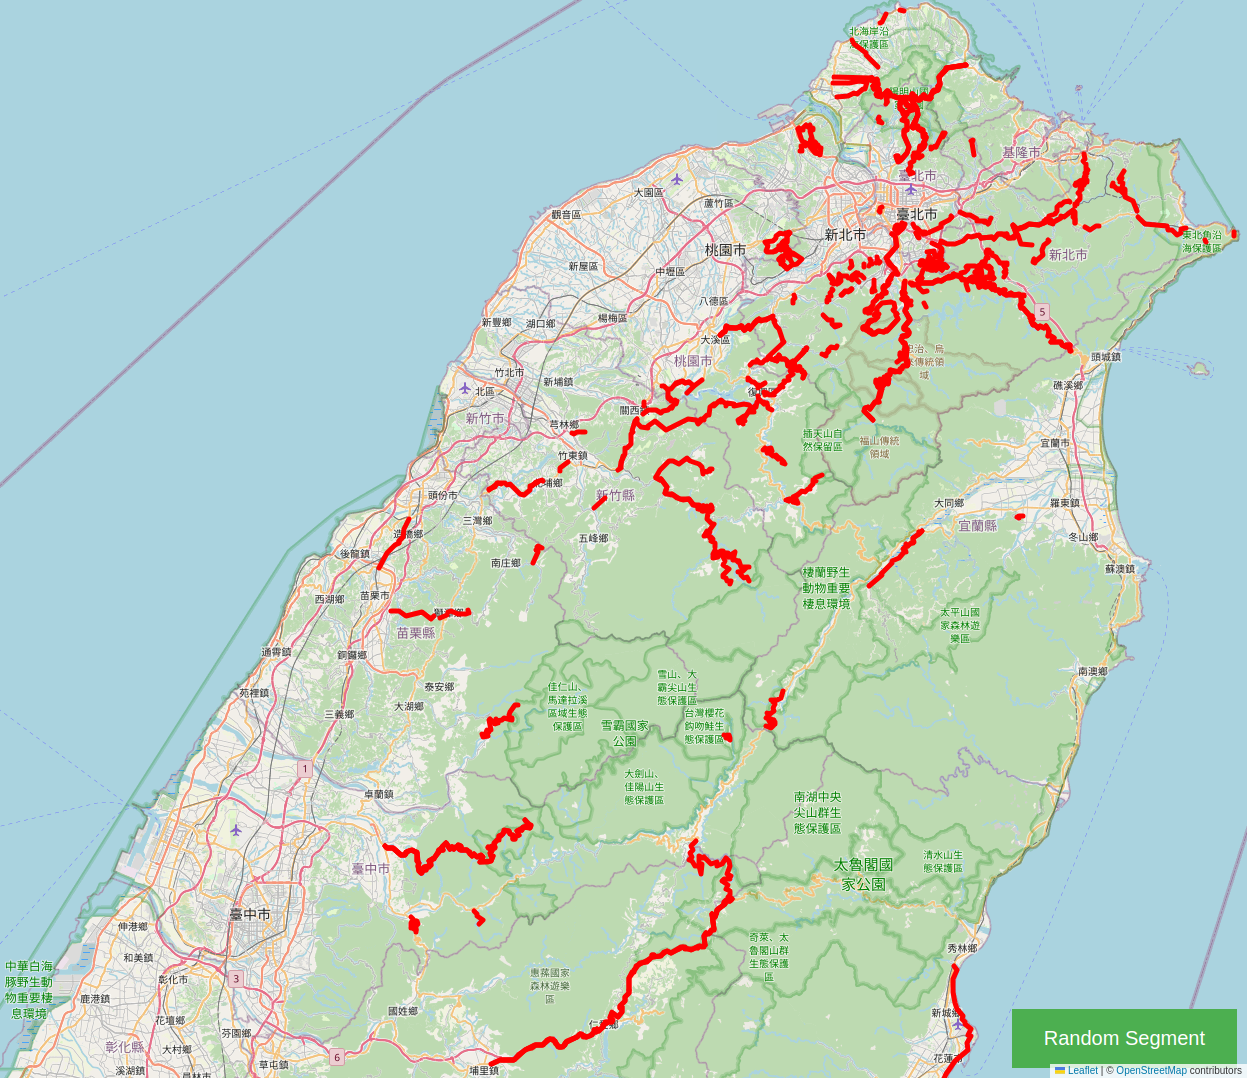
\includegraphics[height=4cm]{segmentHeatMap.png}
\end{frame}
